% !TEX root=report.tex
\subsection{Competitor Sets} \label{subsec:competitor_sets}

The data we received from CouchSurfing does not allow us to know exactly when a host has looked at a couch request, but it does have timestamps for every request and every decision made by a host.
To form sets of ``competing'' requests, we use a heuristic procedure to scan through all requests made to a particular host, and split them into groups based on their timing.

In the following, requests carry the same index as the user/surfer that invoked them, i.e., surfer $s_i$ sends request $c_{i,j}$ to host $h_j$.
In the following examples, $h$ is fixed, so we just denote requests as $c_i$.

We assume a session-based behavior for the user, which means he sits down in front of his computer and checks all new request to his couch every once in a while. There will be several different surfers that want to stay with him in different times
 

%For a given period $\tau$, let $C_{j}^{\tau} = c_1, c_2,\ldots,c_n$ be the requests send to $h$. We hereby assume that if at a certain time host $h$ accepts a request $c_i$ for period $\tau$, she prefers the requesting surfer $s_i$ over all other users whose requests she read that overlap with $\tau$. An efficient sweep-line algorithm to find sets of overlapping requests is depicted in.

\subsubsection{Filter rejects by temporal constraints}
\todo{for tobi: i'm confused---how is what was done above different from this? maybe unite?}

\todo{for tobi: insert reference to \autoref{fig:timeline_view} somewhere.}

Using a very similar technique we can filter rejects that are not actually rejects for the reason of a mismatching surfer. Imagine $h$ gets a request $c_1$ at time $t_1$, accepts this request at time $t_2$ and gets another request $c_2$ for the same period as $c_1$ at $t_3$. If we have that $t_1 < t_2 < t_3$, there is no valid information about whether or not $h$ likes surfer $s_2$. By the time he gets the second request, his couch is already booked out and so he has to reject $s_2$ no matter if he would even prefer him over $s_1$. Because of this scenario we filter our training data for exactly those \textit{uninformative rejects} using again and temporal orderings on requests and acceptances/rejects.

\begin{figure}[ht]
\centering
\subfloat[Requested]{
  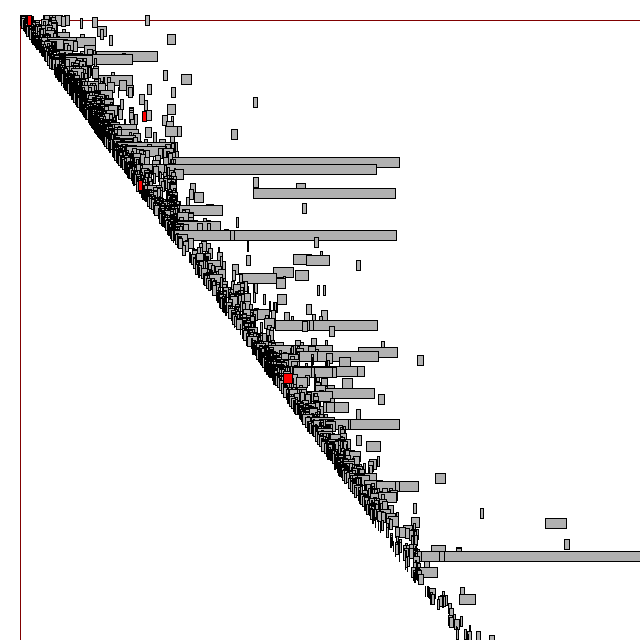
\includegraphics[width=0.45\linewidth]{figures/top_requested.png}
}
\subfloat[Accepted]{
  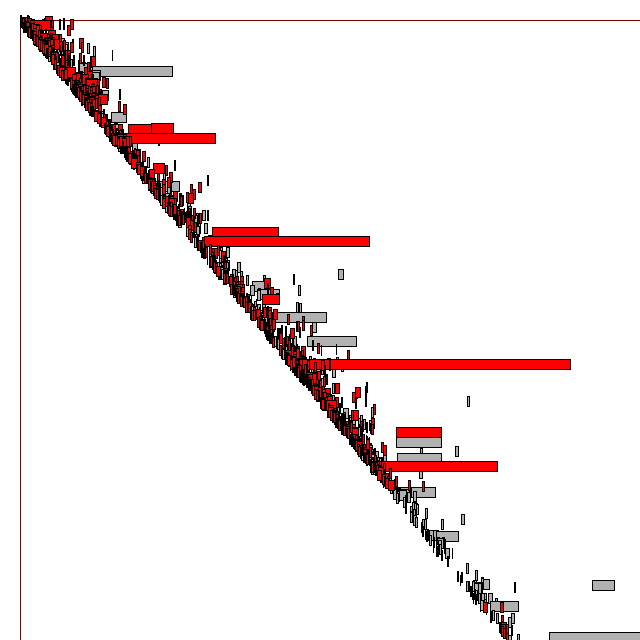
\includegraphics[width=0.45\linewidth]{figures/top_accepted.png}
}
\caption{\todo{for tobi: Explain.}}
\label{fig:timeline_view}
\end{figure}
